\section{Rotations in an actual collar}\label{cr:rotations}

Three proper half-turns will keep track of the order changes:
\begin{equation}\label{cr:rotations-formula}
 \rho(x,y,z)=(-x,-y,z),\quad
 \kappa(x,y,z)=(x,-y,-z),\quad
 \tau(x,y,z)=(-x,y,-z)=\Turn^2(x,y,z).
\end{equation}
Their endpoint permutations are $(01)(23)$, $(03)(12)$ and $(02)(13)$, respectively. Direct composition of these spatial maps gives
\begin{equation}\label{cr:rotation-rules}
\begin{aligned}
 \rho(FG)&=\rho(F)\rho(G),&\rho(\Turn F)&=\Turn\kappa(F),\\
 \kappa(FG)&=\kappa(G)\kappa(F),&\kappa(\Turn F)&=\Turn\rho(F),\\
 \tau(FG)&=\tau(G)\tau(F),&\tau(\Turn F)&=\Turn\tau(F).
\end{aligned}
\end{equation}
The order reverses precisely when the stack coordinate reverses.

Each standard integral braid is fixed by these half-turns, with its signed exponent unchanged. One direct model has its two strand positions at height $z\in[-1,1]$ proportional to
\[
 \pm\bigl(\cos(\pi n(z+1)/2),\sin(\pi n(z+1)/2)\bigr)
\]
in the transverse plane, after a fixed choice of sign convention. Each map in \eqref{cr:rotations-formula} changes the displayed angle only by an integral multiple of $\pi$ after the prescribed height reversal. The unordered pair of strands is therefore unchanged. The same conclusion holds for $h_i=\Turn R^{n_i}$ by \eqref{cr:rotation-rules}. Reversal in the projection is accompanied by the necessary reversal of depth; it does not negate a crossing. Pushing a half-turn through an expression consequently reverses specified product orders but preserves all leaf labels and weights.

\begin{lemma}[Twist sliding]\label{cr:slide}
For every tangle $F$, including its closed components, and every $a,b\in\mathbb Z$,
\begin{equation}\label{cr:slide-formula}
 R^aF\simeq\rho^a(F)R^a,\qquad
                     R^aR^b\simeq R^{a+b}.
\end{equation}
The first isotopy is relative to the four outside endpoints. The symbol $\simeq$ denotes an ambient isotopy, carrying a marked point and any chosen ribbon.
\end{lemma}
\begin{proof}
Put $F$ in a smaller round cylinder inside the box and leave empty collars at both ends. In cylindrical coordinates $(r,\phi,z)$, take smooth cutoffs $\eta(r),\xi(z)$ equal to one on that smaller cylinder and zero near the outside boundary. The maps
\[
 (r,\phi,z)\longmapsto
            (r,\phi+t\pi\eta(r)\xi(z),z),\qquad0\le t\le1,
\]
are homeomorphisms fixed near the boundary: their inverse subtracts the same angle since $r,z$ are unchanged. At the end the inner tangle has rotated by $\rho$. Its two end collars acquire opposite half twists. Choose the angle sign to match $R$. Applying this isotopy to $\rho(F)$ yields $R F\simeq\rho(F)R$. The inverse isotopy and iteration prove the formula for all $a$. Closed components lie inside the rotating cylinder and move with it. The second assertion concatenates equal twists and cancels adjacent opposite crossings by Reidemeister II.
\end{proof}

The rotation $\rho^a$ depends only on $a\bmod2$. An integral factor can thus be moved through an ordered stack, but every factor passed acquires its stated rotation. There is no assertion that open factors commute.

\section{The closing sphere and its ordered moves}\label{cr:closing}

The four connections in $C(FG)$ are exactly
\begin{equation}\label{cr:closing-pairs}
 F_2\leftrightarrow G_1,\quad F_3\leftrightarrow G_0,
 \quad F_0\leftrightarrow G_3,\quad F_1\leftrightarrow G_2.
\end{equation}
The first two are the stack collar and the last two are the empty outside arcs. Straightening these collars with their planar sectors identifies the two tangle-ball boundaries by
\begin{equation}\label{cr:reflection}
            h(x,y,z)=(x,y,-z),\qquad h(i)=3-i.
\end{equation}
This is orientation reversing on the sphere. Although its endpoint permutation equals that of $\kappa$, it is not the proper rotation $\kappa$.

\begin{lemma}[Closed turns and cyclicity]\label{cr:closed-moves}
For the fixed closures,
\begin{align}
 C((\Turn F)G)&\simeq C(F(\Turn G)),\label{cr:turn-transfer}\\
 C((\Turn F)(\Turn G))&\simeq C(F\tau(G)),\label{cr:double-turn}\\
 C(FG)&\simeq C(GF).\label{cr:cyclic}
\end{align}
All rotations on the right are actual rotations of the indicated tangles.
\end{lemma}
\begin{proof}
Let $\Turn_t$ be rotation through $t\pi/2$ in the diagram plane. The specified gluing has
\[
                     h\Turn_t h^{-1}=\Turn_t^{-1}.
\]
Act by $\Turn_t$ on the first ball and by $\Turn_t^{-1}$ on the second. These maps agree under the boundary identification and extend over the balls. They give an isotopy of their glued $S^3$, starting at the identity. Applied to $C(F(\Turn G))$, its endpoint at $t=1$ is $C((\Turn F)G)$. This proves \eqref{cr:turn-transfer}; substituting $\Turn G$ for $G$ gives \eqref{cr:double-turn}. A boundary Dehn twist not present in \eqref{cr:closing-pairs} would change this argument.

For cyclicity put the two successive stack intervals in the standard unknotted solid torus $D^2\times S^1$ and move the cutting section past the first interval. Translation around its circle coordinate gives the isotopy. In the model $S^3\subset\mathbb C^2$, rotation of the corresponding complex coordinate extends this translation to the ambient sphere. The marked point and every component are carried along. This proves only closed cyclicity, as used here.
\end{proof}

\begin{lemma}[Exposing a leaf or junction]\label{cr:expose}
In a cylindrical product closure with at least two labelled leaves, any chosen leaf can be exposed as $C(h_iQ)$. Every other leaf occurs in $Q$ exactly once. Likewise any chosen product junction can be brought to the closing sphere, with its original attached subexpressions in recorded order.
\end{lemma}
\begin{proof}
Regard a selected subtree as the first argument of $C(AQ)$. If $A=BC$ and the target lies in $B$, reassociate to $C(B(CQ))$. If it lies in $C$, use cyclicity to obtain $C(C(QB))$. If $A=\Turn B$, transfer the turn to obtain $C(B(\Turn Q))$. Start by cyclicity if the target lies in the other closing factor. Each step shortens the path to the selected leaf or junction and moves a sibling, never copies it. Stop at that target. Orders and all new turns are given explicitly by these formulas.
\end{proof}

\begin{figure}[ht]
\centering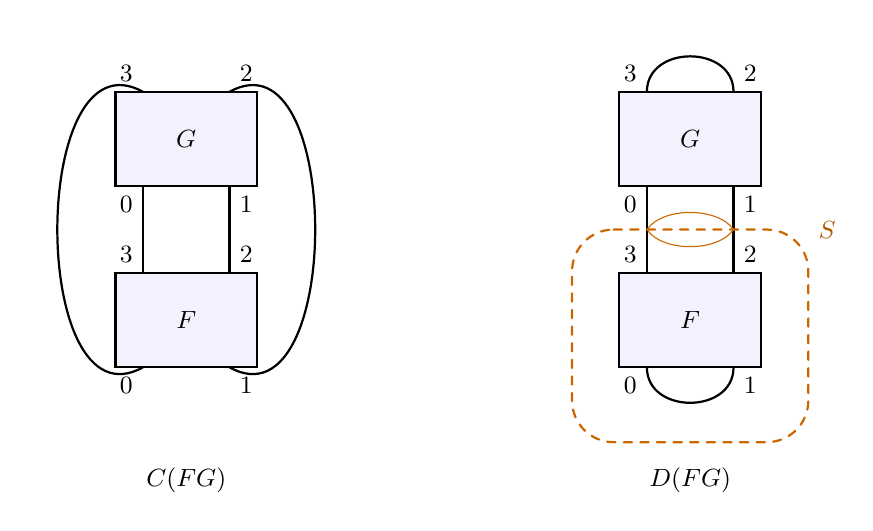
\begin{tikzpicture}[x=1cm,y=1cm,line cap=round,thick,
 every node/.style={font=\small}]
\foreach \dx/\lab in {0/{C(FG)},6.4/{D(FG)}}{
 \begin{scope}[shift={(\dx,0)}]
 \draw[fill=blue!5] (-.9,0) rectangle (.9,1.2);
 \draw[fill=blue!5] (-.9,2.3) rectangle (.9,3.5);
 \node at (0,.6) {$F$};\node at (0,2.9) {$G$};
 \foreach \x in {-.55,.55}{\draw (\x,1.2)--(\x,2.3);}
 \node[below] at (0,-1.15) {$\lab$};
 \node[below left] at (-.55,0) {$0$};
 \node[below right] at (.55,0) {$1$};
 \node[above right] at (.55,1.2) {$2$};
 \node[above left] at (-.55,1.2) {$3$};
 \node[below left] at (-.55,2.3) {$0$};
 \node[below right] at (.55,2.3) {$1$};
 \node[above right] at (.55,3.5) {$2$};
 \node[above left] at (-.55,3.5) {$3$};
 \end{scope}
}
\draw (-.55,0).. controls (-2,-.8) and (-2,4.3)..(-.55,3.5);
\draw (.55,0).. controls (2,-.8) and (2,4.3)..(.55,3.5);
\draw (5.85,0)..controls(5.85,-.6)and(6.95,-.6)..(6.95,0);
\draw (5.85,3.5)..controls(5.85,4.1)and(6.95,4.1)..(6.95,3.5);
\draw[orange!80!black,dashed,rounded corners=15pt]
 (4.9,1.75)--(7.9,1.75)--(7.9,-.95)--(4.9,-.95)--cycle;
\node[right,orange!70!black] at (7.9,1.75) {$S$};
\draw[orange!80!black,thin] (5.85,1.75)..controls(6.05,1.46)and(6.75,1.46)..(6.95,1.75);
\draw[orange!80!black,thin] (5.85,1.75)..controls(6.05,2.04)and(6.75,2.04)..(6.95,1.75);
\end{tikzpicture}

\caption{The prescribed closures of the same lower box $F$ and upper box $G$. The cylindrical closure on the left uses the outside returns of \eqref{cr:closing-pairs}. For the cap closure on the right, a sphere around $F$ and its lower cap meets only the two interface strands. The dashed line is the section of that sphere in the diagram plane. Cutting there creates the upper cap of $F$ and the lower cap of $G$, so the connected-sum components are specified. Endpoint numbers refer to each box before stacking.}\label{cr:closure-figure}
\end{figure}
